% !TeX spellcheck = en_US
% !TeX root = ./0_article.tex

\section{Body Biasing Injection: disturbances nature and propagation}
\IEEEPARstart{S}{imulating} a fault injection method behavior is an important part in understanding its mechanisms.
Whether it is EMFI, LFI or BBI, it allows predicting and understanding the underlying phenomena at work to set up reliable experiments.

Ideally, we would want to directly observe signals inside integrated circuits, allowing for fine measurements of power supply voltages, currents, and logic levels at a transistor-level.
However, embedding sensors into an already existing IC is not possible, and doing so on future IC is costly, takes time to fully implement, and requires the manufacturer to do so.
In addition to this, we do not have any guarantee that these sensors will not be disturbed too much by the fault injection.
Therefore, we have decided to take the following approach:
\begin{center}
%	Simulation \textrightarrow\ Conclusions \textrightarrow\ Verification
	Simulation \textrightarrow\ Analysis \textrightarrow\ Hardware Verification
\end{center}

By doing so, we have freed ourselves from hardware limitations.
However, other limitations remains.
Indeed, modern ICs, even the smallest, embed millions of transistors, and with current technologies, it is impossible to evaluate with simulations entire circuits at a transistor level.
Therefore, to tackle these limitations, we decided to adopt an hybrid approach, combining transistor-less models and local logic gates simulations.
This approach is a compromise between accuracy and computational cost/time, and allows simulating relatively big circuits under BBI disturbances
Overall, it is similar to what has been done for EMFI in \cite{mathieuEMFI}.
The resulting simulation flow is divided in three consecutive steps:
\begin{itemize}
	\item The simulation of an IC under BBI using a transistor-less model, allowing for a purely electrical analysis;
	\item The extraction of significant disturbed power signals from the previous simulation;
	\item The simulation of functional logic gates under BBI thanks to the previously extracted signals.
\end{itemize}

%\subsection{An hybrid simulation flow: building the models}
\subsection{Modeling ICs and BBI platforms}
	Building the correct models for the simulation flow pass through multiple steps.
	As the goal of the hybrid flow is to reduce the computational time required to evaluate an IC, it is still important to maintain a certain accuracy concerning the IC physical structure.
	To do so, the models are designed around actual IC implementations.
	The main building blocks of the models are the power supply network, the standard-cells, and the substrate structure.
	In this work, we are only focusing on bulk substrates: specifically dual-well and triple-well substrates.

	\subsubsection{Power supply rails and standard-cell segments}
		% !TeX spellcheck = en_US
% !TeX root = ./0_article.tex
% LABEL AFTER CAPTION WESH GEOFFREY !!
\begin{figure}[h]
	\centering
	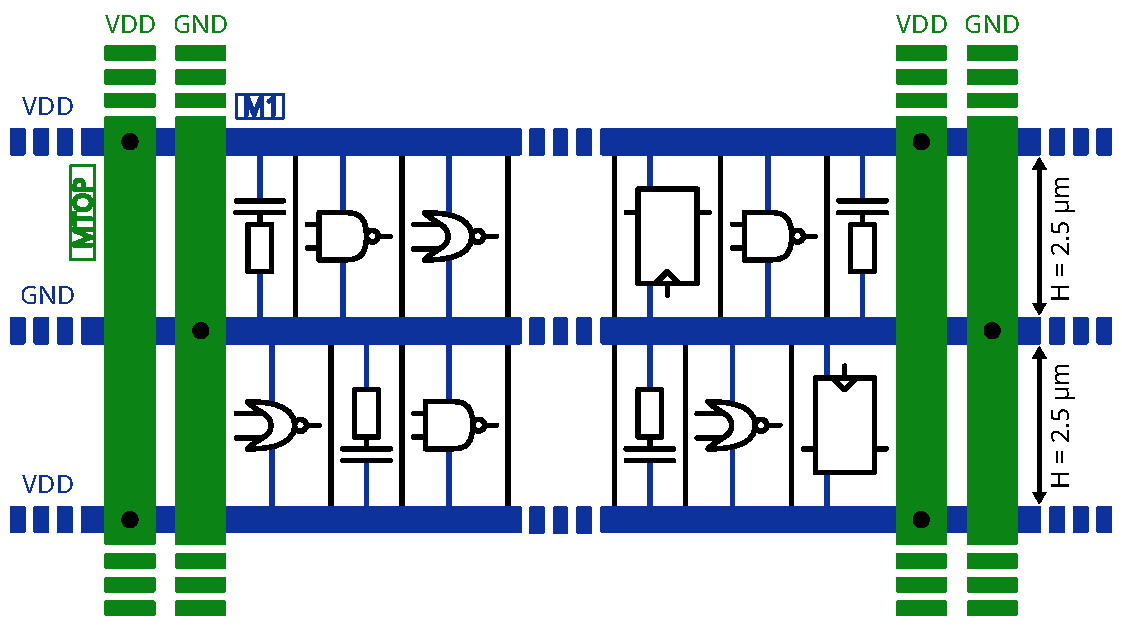
\includegraphics[width=0.49\textwidth]{./figures/psu_std_cell.pdf}
	\caption{A Standard-Cell Segment and its power delivery network.}
	\label{fig_alim_std}
\end{figure}

		The power distribution inside an IC is typically made with a grid-like structure, composed of metal wires stacked on top of each other on planes.
		In each layer, the metal wires are equally spaced and have a dedicated width, which becomes thinner the deeper they are.
		The lowest layer brings the power directly to the transistors.
		Fig. \ref{fig_alim_std} presents a common power delivery network, designed with two metal levels for simplicity (in blue and green).

		Within the metal lines are located standard-cell segments (SCS), composed of decoupling, logic and sequential elements, and are pre-characterized by foundries and categorized depending on their performance (mainly but not exclusively power consumption and speed).
		As illustrated in Fig. \ref{fig_alim_std}, SCS have a constant height, in our case of 2.5 \textmu m, and a variable width depending on how much logic gates each one of them embed.
		As we have stated previously, the hybrid simulation flow use transistor-less models as basic IC building blocks.
		Therefore, the transistors, hence the standard-cell segments, are modeled with passive elements such as resistors and capacitors.

		% !TeX spellcheck = en_US
% !TeX root = ./0_article.tex

\begin{figure}[h]
	\centering
	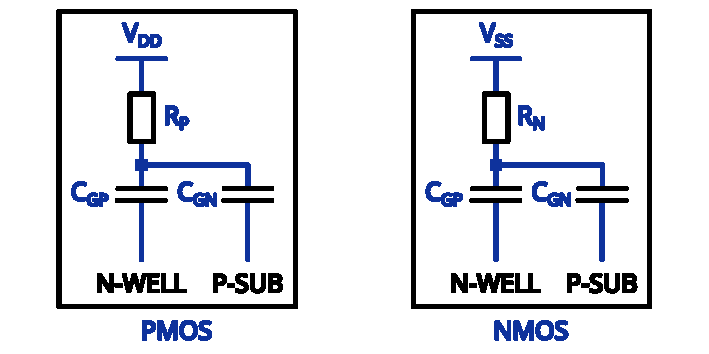
\includegraphics[width=0.9\columnwidth]{./figures/std_cell_logic_passive.pdf}
	\caption{Transistor-less equivalent model of a set of PMOS and NMOS in a SCS.}
	\label{mos_passive}
\end{figure}

		To that end, the elementary SCS chosen measures 30 \textmu m by 5 \textmu m, representing two rows of logic cells.
		This represents about a hundred of logic gates, represented with four resistors and two capacitors, as shown in Fig. \ref{mos_passive}, with half of the transistors conducting, half not conducting.
	%	Respectively, the conducting NMOS and PMOS transistors, whose source is respectively connected to $V_{SS}$ and $V_{DD}$ are respectively equivalent to a passive resistor $R_N$ and $R_P$.
		The conducting NMOS transistors, whose source is connected to $V_{SS}$, are equivalent to the passive resistor $R_N$.
		The conducting PMOS transistors, whose source is connected to $V_{DD}$, are equivalent to the passive resistor $R_P$.
		The resistors values depends on the considered technology, as well as the capacitors values, and can be adjusted and calculated according to one needs.

	\subsubsection{The substrate}
		% !TeX spellcheck = en_US
% !TeX root = ./0_article.tex

\begin{figure}[h]
	\centering
	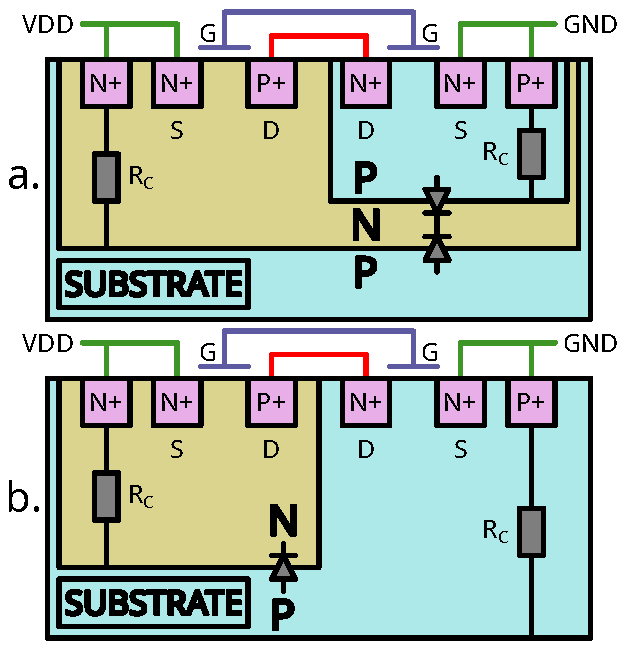
\includegraphics[width=0.35\textwidth]{./figures/substrate_2.pdf}
	\caption{Triple-well (a) and Dual-well (b) inverter cross-sectional view.}
	\label{fig_sub}
\end{figure}

		Because BBI can be performed thanks to the silicon substrate as the main physical environment transferring energy from a generator to an IC, it is fundamental to elaborate a proper substrate model to precisely represent the various involved phenomena.
		As stated previously, our work focuses on bulk substrates, and in most cases, the substrate silicon is P-doped.
		There are two typical ways of lithographing the transistors in a bulk substrate, using dual-well or triple-well structures.
		Dual-well substrates are commonly found in moderately old circuits, while triple-well substrate is found mixed with dual-well in more recent circuits, while not bleeding-edge.

		To properly understand how the differences between dual-well and triple-well substrates change the resulting model, let us analyze the cross-sectional schematics of an inverter created respectively in a triple-well and a dual-well substrate, as shown respectively in Fig. \ref{fig_sub}.a and Fig. \ref{fig_sub}.b:
		\begin{itemize}
			\item In the triple-well substrate, the NMOS transistors are lithographed into a P-doped silicon well, itself lithographed inside a N-doped well, buried inside the P-doped substrate. The PMOS transistors are located inside the N-doped well;
			\item In the dual-well substrate, the PMOS transistors are still located inside the N-doped well, however, the NMOS are lithographed directly inside the P-doped substrate.
		\end{itemize}
		On the one hand, the triple-well substrate reveals two diodes:
		\begin{itemize}
			\item One formed between the P-well and the N-well;
			\item Another formed between the N-well and the P-substrate.
		\end{itemize}
		On the other hand, the dual-well substrate only reveals one diode between the N-well and the P-substrate.

	\subsubsection{The resulting model}
		Thanks to what we have introduced previously, we can now build the elementary building blocks for our hybrid simulation flow.
		It combines the power delivery network architecture, the equivalent logic gates models, and the substrate structure, all in an embedded model.
		This model represents an elementary section of the simulated IC, measuring 30 \textmu m by 5 \textmu m by $t_{Sub}$ \textmu m, the latter being the substrate thickness, a parameter which will vary depending on each considered IC.
		% !TeX spellcheck = en_US
% !TeX root = ./0_article.tex

\begin{figure*}[ht]
	\centering
	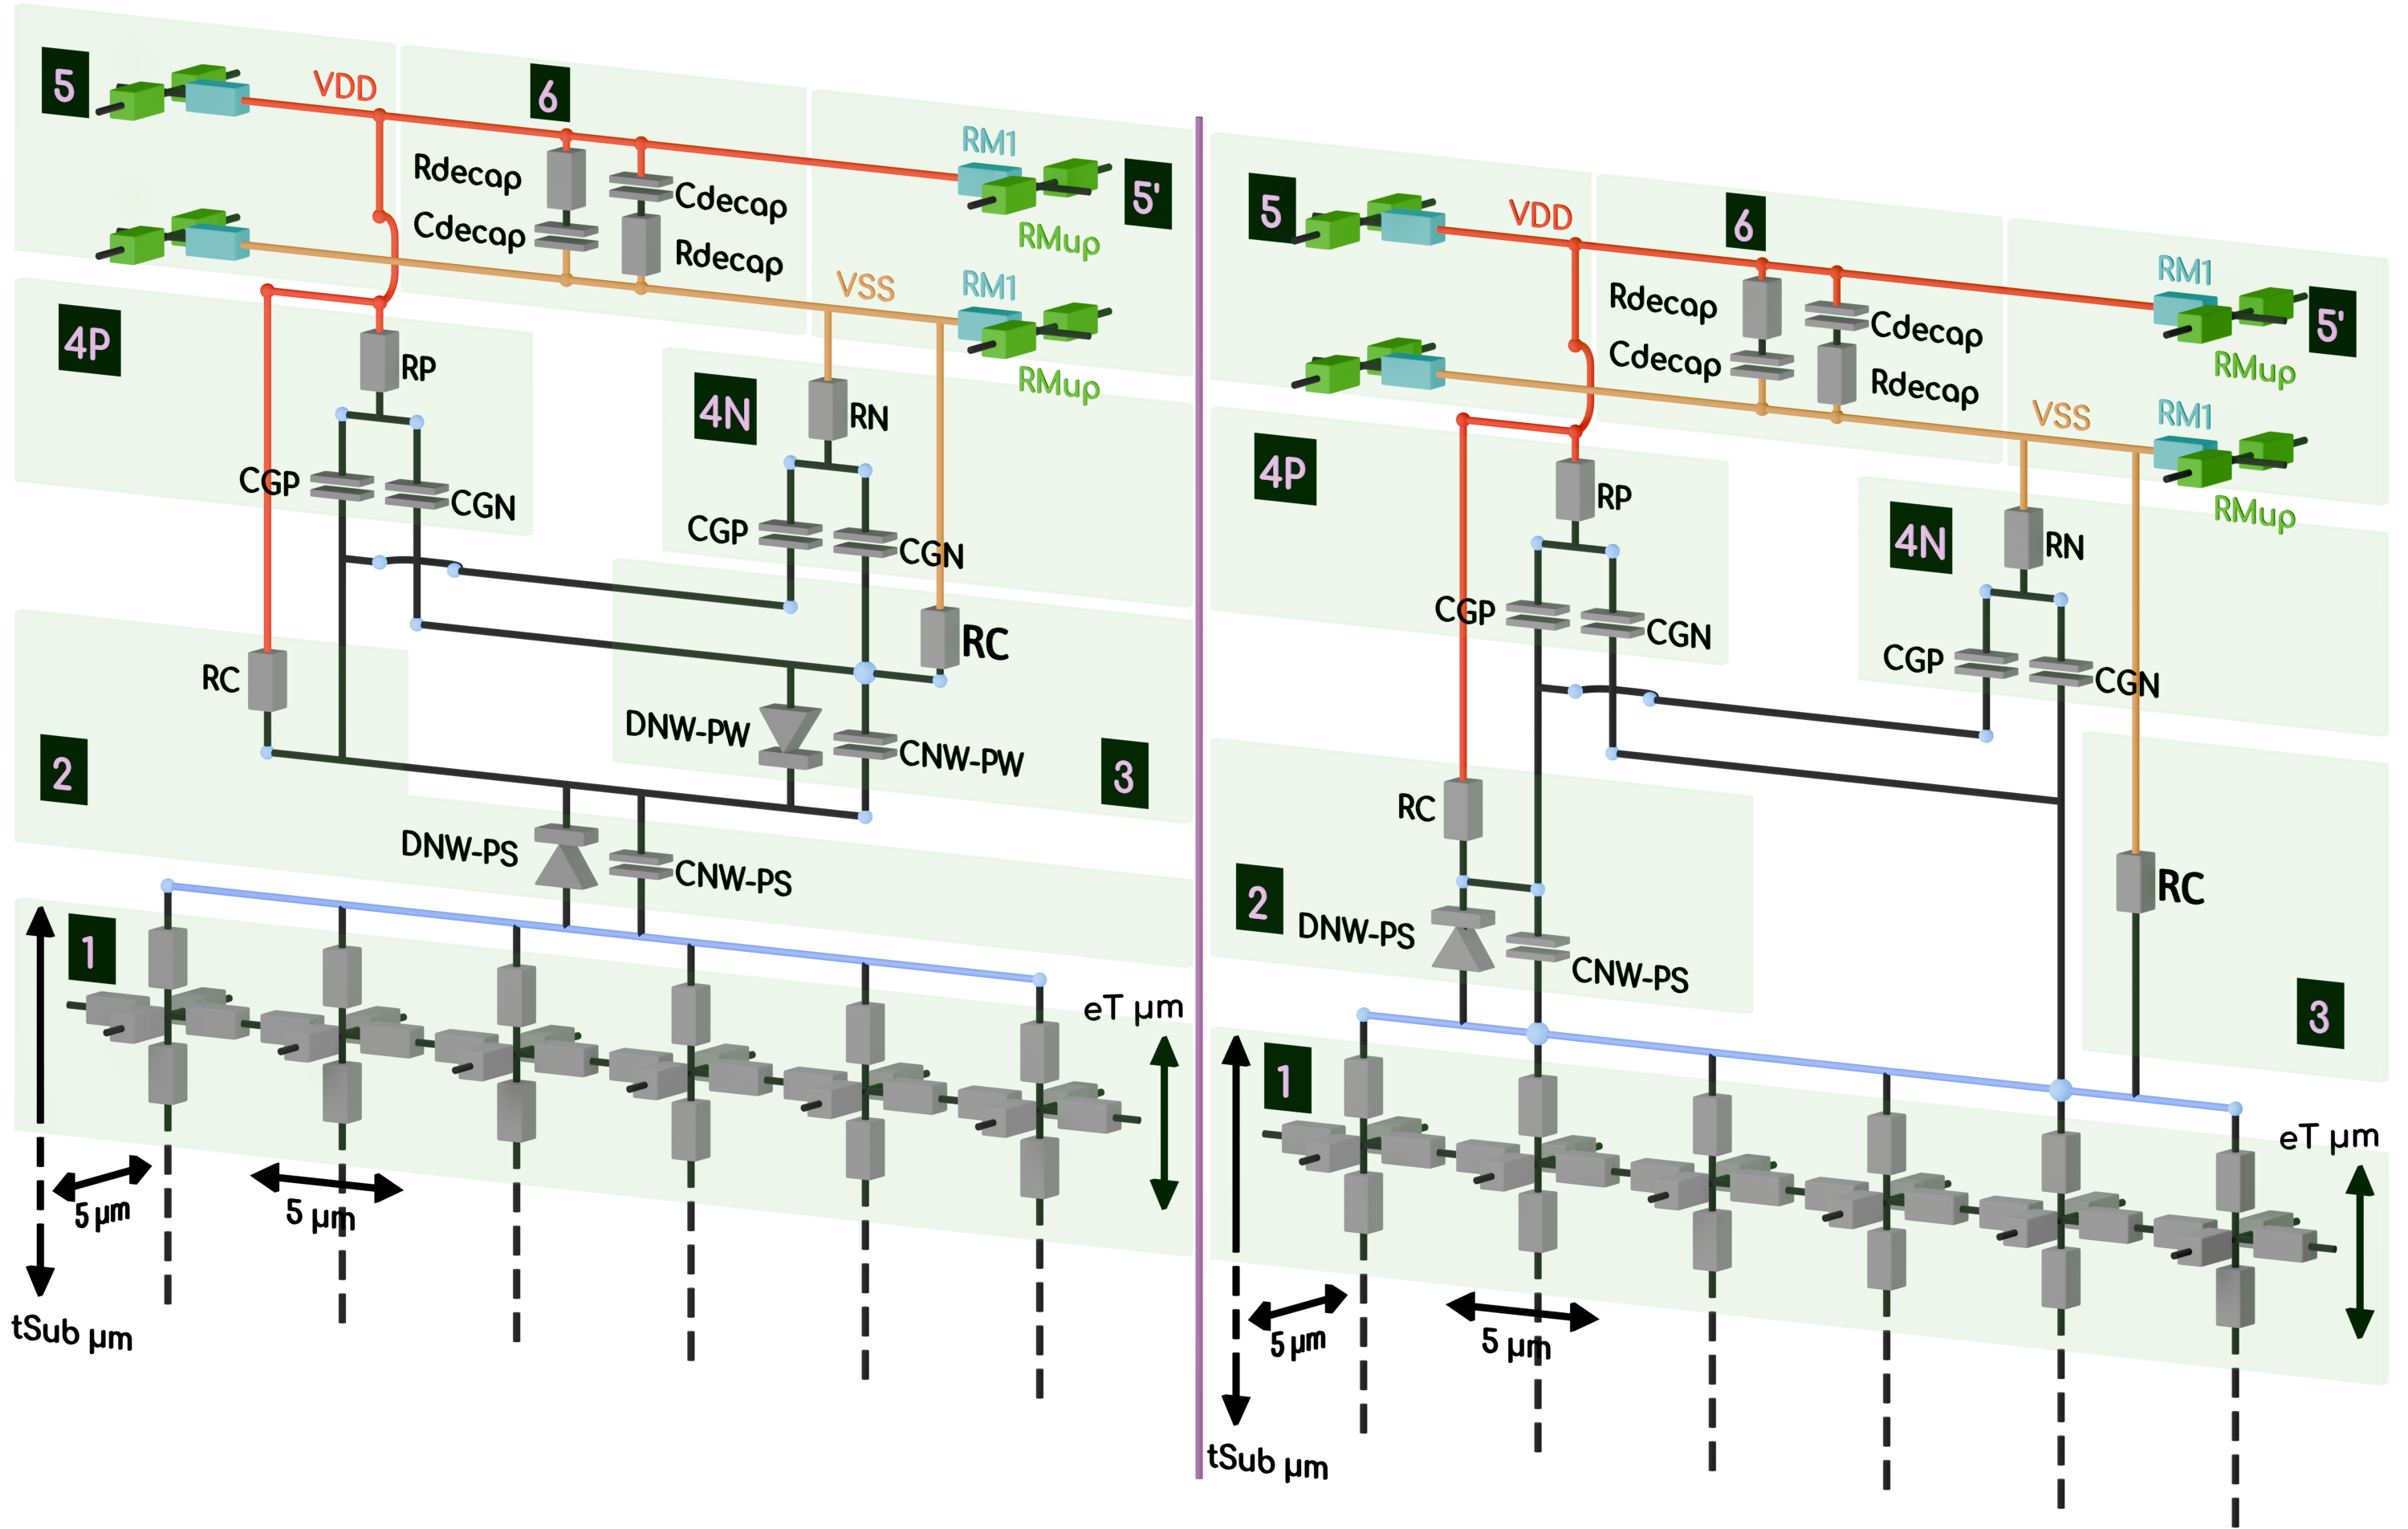
\includegraphics[width=0.95\textwidth]{./figures/dual+triple3.png}
	\caption{Triple well (left) and dual well (right) std cell \textcolor{red}{(PEUT ETRE FAIRE DES SOUS-FIGURES)}}
	\label{fig_triplewellstdcell}
\end{figure*}

		As we consider both triple-well and dual-well substrate, there are two resulting elementary models, shown in Fig. \ref{fig_triplewellstdcell}.
		Each model is composed of various sub-regions, whose descriptions follow:
		\begin{itemize}
			\item \ovalbox{1} is the substrate network, divided into six sub-networks of six resistors for finer details;
			\item \ovalbox{2} is the first P-N silicon junction, common to both models;
			\item \ovalbox{3} is the access resistor (DW) or the second junction (TW);
			\item \ovalbox{4P} is the PMOS equivalent section;
			\item \ovalbox{4N} is the NMOS equivalent section;
			\item \ovalbox{5, 5'} are the power supply metal layers (upper metal in green, first level in blue);
			\item \ovalbox{6} is the power supply decoupling.
		\end{itemize}
		As we have stated before, these models only represent a small portion of the modeled IC.
		To create an entire IC of a defined size, it is required to instantiate and interconnect as much as needed the elementary models.
		By doing so, we can create a bigger model of virtually any size.
		The language we have chosen to work with the simulation is the SPICE language.
		However, we created a custom Python script to interconnect the SCS together, place external power connections, and generate a SPICE file.
		For the current work, we decided to put the external power connections at the top and bottom of the IC (seen from above), and the BBI probe at the center of the IC (on the backside).

%\subsection{An hybrid simulation flow: performing simulations}
\subsection{Simulation results: operating point}
	Now that we set up the base models and their duplication, we can perform simulations with those models.
	To properly use these models, it is required, in the first place, to validate them through various steps to ensure their reliability.
	To that end, we generated an IC measuring 550 \textmu m by 450 \textmu m with a 140 \textmu m substrate thickness, and performed an operating point to verify the correctness of the models for each substrate type.
	% !TeX spellcheck = en_US
% !TeX root = ./0_article.tex

\begin{table}[H]
	\label{tab_op}
	\centering
	\begin{tabular}{lll}
		Value  & Triple-well & Dual-well \\ \hline
		$I_{GND}$                               & 2 nA          & 2.2 nA    \\
		$I_{VDD}$                                & -7 nA        & 3 nA        \\
		$\overline{GND_{drop}}$    & 2 nV         & 2 nV        \\
		$\overline{V_{DD_{drop}}}$    & 3 nV         & 3 nV       
	\end{tabular}
	\caption{op point}
\end{table}

	We should expect almost no voltage drop and zero current consumption from such a model.
	Otherwise, it indicates an underlying issue with the model.

	Table \ref{tab_op} shows the operating point results for both a triple-well and a dual-well circuit, and indicates a correct operating point, with idle currents and voltage drops close to zero.
	However, verifying the bias point alone is not sufficient to consider the model validated.
	As these models are dedicated to be mainly used in transient simulations, it is required to perform one and evaluate the soundness of its results.

	Therefore, we performed transient simulations with a triple-well and dual-well IC, with the following parameters:
	\begin{itemize}
		\item A nominal power supply voltage of 1.2 V;
		\item A voltage pulse amplitude of \textpm\ 300 V;
		\item A voltage pulse width of 15 ns;
		\item Rise and fall times of 8 ns;
		\item A simulation duration of 80 ns;
		\item A simulation time step: of 50 ps.
	\end{itemize}

%\subsection{An hybrid simulation flow: analyzing the results}
	Analyzing the simulation results involves observing various internal IC signals, for each substrate type, the ones presented in this section being:
	\begin{itemize}
		\item The power supply voltage distribution;
		\item The epitaxial current;
		\item The substrate current distribution;
		\item The substrate per-layer current density.
	\end{itemize}
	The observed signals are displayed in two dimensions and at the apex of the BBI disturbance.
	Each signal brings some insights on what happens inside the circuits during a BBI pulse.
	We will first analyze the dual-well results, then the triple-well ones, to finally conclude with a comparison of both.
	% !TeX spellcheck = en_US
% !TeX root = ./0_article.tex

\begin{figure}[ht]
	\centering
	\begin{subfigure}[t]{0.48\columnwidth}
		\includegraphics[width=\textwidth]{imagefile}
		\caption{text}
		\label{key}
	\end{subfigure}
\end{figure}
%	\subsubsection{Negative dual-well simulation results}
	\subsection{Simulation results: dual-well negative pulse}
		Fig. \ref{sim_res_dw_neg} shows the dual-well positive pulse results.

		Sub-fig. left \ref{sim_res_dw_neg}a represents the power delivery network (PDN) voltage across the entire IC as seen from above.
		In other words, it is the supply voltage of the transistors.
		Expectedly, far from the external power connections, we observe some deviation from the nominal 1.2 V power supply voltage.
		However, at the center of the circuit, in other words under the BBI probe, the voltage goes up to 2.8 V, being a 33 \% increase from the nominal value.

		To put these values into perspective, let us look at sub-fig. right \ref{sim_res_dw_neg}a, showing the epitaxial current distribution, representing the charges going from the substrate to the top of the SCS.
		According to the sub-figure, most of the charges are flowing at the center of the IC, under the BBI probe, as the current is the highest in that location.
		It is sound when comparing left and right sub-fig. \ref{sim_res_dw_neg}a, as the voltage difference from the nominal value is higher where the epitaxial current is higher.

		Sub-fig. \ref{sim_res_dw_neg}b and sub-fig. \ref{sim_res_dw_neg}c both represent the same physical quantity in two different ways.
		We have chosen this approach to extract as much information as possible from these models and simulations.
		Sub-fig. \ref{sim_res_dw_neg}b shows the cross-sectional view (from the Y-axis) of the current distribution inside the silicon substrate.
		The substrate being an isotropic environment, in other words, its resistivity is homogeneous in every spatial directions, we can observe a hemispheric current distribution in it.
		However, due to the large difference between the first layer (the farthest to the probe) and the last layer (the closest to the probe), it is difficult to do more observations.
		Therefore, we can look at sub-fig. \ref{sim_res_dw_neg}c, which represents the same data in a different perspective.
		To better illustrate the inter-layer differences, we have chosen to normalize the data in a per-layer basis.
		Thus, it allows us to compare the current density between layers.
		It is important to note that the normalized values are calculated in a way that the closer they are to zero, the denser the current is, and vice-versa.
		The layer 0 is the closest to the logic gates, while the layer 13 is the closest to the backside (the probe).
		What is interesting to note here is that for each substrate layer, the current is focused where the probe is located.
		It is to be expected, as the substrate is isotropic.
		However, the deeper we are into the substrate, the less focused the current is.
		Once again, it is quite logical as the charges diffuse homogeneously inside the substrate.

	\subsection{Simulation results: dual-well positive pulse}
		Concerning the positive pulse dual-well results, let us look at Fig. \ref{sim_res_dw_pos}.
		Compared to the previous results, sub-fig. left \ref{sim_res_dw_pos}(a) shows that the PDN voltage exhibits not a voltage increase, but rather a voltage drop.
		Indeed, under the probe, the PDN voltage drops to 500 mV from 1.2 V.
		This is a substantial difference, which could lead, if applied to actual transistors, a significant change in behavior such as an incorrect biasing.

		Concerning the epitaxial current, shown in sub-fig. right \ref{sim_res_dw_pos}a, we can notice two key changes.
		First, the current polarity has changed, from a negative to a positive one.
		Once again, it was to be expected, as the voltage pulse polarity has changed.
		Then, in absolute value, the maximal current is 500 mV higher than previously, which indicates that more energy has been injected into the circuit.
		Eventually, regarding the substrate current, there are no major differences except the current polarity, both for sub-fig. \ref{sim_res_dw_pos}b and sub-fig. \ref{sim_res_dw_pos}c.

	\subsection{Simulation results: triple-well negative pulse}
		Let us take a closer look at Fig. \ref{sim_res_tw_neg}.
		These results stand out all of the others, in many ways.
		First, if we take a look at sub-fig. left \ref{sim_res_tw_neg}(a) regarding the PDN voltage, we can see that there are very little variations from the nominal voltage.
		Indeed, the voltage drops only to 1.1 V.
		Then, concerning the epitaxial current shown in sub-fig. right \ref{sim_res_tw_neg}a, we can see that it is almost a hundred times lower than on other results.
		It is then confirmed in sub-fig. \ref{sim_res_tw_neg}(c) with the substrate current distribution.
		However, the current density stays consistent with the previous results.
		Before analyzing further these results and explaining them, let us analyze the last case.

	\subsection{Simulation results: triple-well positive pulse}
		Quite interestingly, with a triple-well substrate and a positive voltage pulse, as displayed in Fig. \ref{sim_res_tw_pos}, we observe results that are very similar to the dual-well negative case (Fig. \ref{sim_res_dw_neg}), whether it is on the PDN voltage or on the epitaxial current.
		Indeed, the PDN voltage disturbance is almost identical to sub-fig. left \ref{sim_res_dw_neg}a, with an increase in voltage from 1.2 V to 2.8 V.
		Then, the epitaxial and substrate current maps are mirrors (in polarity) of sub-fig. left \ref{sim_res_dw_neg}a and \ref{sim_res_dw_neg}c.
		Eventually, the current density graph is very close to the other results.

%	\subsubsection{Differences between dual-well and triple-well (negative and positive pulses)}
	\subsection{Simulations results: summary and conclusions}
		As we have seen through this section, we have four possible scenarios:
		\begin{itemize}
			\item A dual-well substrate and a negative voltage pulse;
			\item A dual-well substrate and a positive voltage pulse;
			\item A triple-well substrate and a negative voltage pulse;
			\item A triple-well substrate and a positive voltage pulse.
		\end{itemize}
		Each scenario behave differently than the others for one main reason: the electric coupling between the probe (substrate) and the SCS (logic).
		These differences in coupling are due to the substrate structure we encounter in dual-well and triple-well circuits.

		As we have described before, the dual-well substrate embeds a P-N diode between the P-substrate and the N-well, and depending on the voltage pulse polarity, this diode is either blocking or conducting.
		This diode is interspersed between the substrate and the PMOS section.
		On the one hand, concerning the negative pulse scenario, the diode is blocking, thus creating an AC-coupling between the probe and the PMOS.
		On the other hand, the NMOS are DC-coupled to the probe as they are connected through a resistive path.
		Therefore, the circuit is globally DC-coupled to the probe, allowing the charges to flow all the time during the pulse.
		Then, concerning the positive pulse scenario, the diode conducts, creating another DC path to the transistors, reducing the effective circuit impedance seen by the probe.
		It explains the greater observed currents, as the charges have an additional DC path to follow.

		On the triple-well side, the top of the SCS is barred with a first P-N diode (P-substrate N-well), and the NMOS are behind another diode.
		When using negative pulses, the first diode is blocking, therefore creating a pure AC-coupling between the probe and the circuit.
		It means that the charges are able to flow in and out of the SCS only on the pulse edges.
		Consequently, for a given voltage pulse, less energy is transferred into the IC in that case.

		Then, regarding the triple-well positive scenario, the first diode become conducting, while the second stays blocking.
		Therefore, the PMOS are DC-coupled, while the NMOS stay AC-coupled.
		We come back to a scenario similar to dual-well negative.

		% !TeX spellcheck = en_US
% !TeX root = ./0_article.tex

\begin{table}[]
	\centering
%	\resizebox{\columnwidth}{!}{
		\begin{tabular}{
				>{\columncolor[HTML]{EFEFEF}}c
				>{\columncolor[HTML]{EFEFEF}}c cc
				>{\columncolor[HTML]{FFFC9E}}c c}
			\cellcolor[HTML]{DAE8FC}                            & \cellcolor[HTML]{DAE8FC}                           & \multicolumn{3}{c}{\cellcolor[HTML]{DAE8FC}Coupling}                                                                                    & \cellcolor[HTML]{DAE8FC}                           \\
			\multirow{-2}{*}{\cellcolor[HTML]{DAE8FC}Substrate} & \multirow{-2}{*}{\cellcolor[HTML]{DAE8FC}Polarity} & \cellcolor[HTML]{DAE8FC}NMOS                      & \cellcolor[HTML]{DAE8FC}PMOS                      & \cellcolor[HTML]{DAE8FC}Circuit & \multirow{-2}{*}{\cellcolor[HTML]{DAE8FC}Danger}   \\
			Dual-well                                           & Negative                                           & \cellcolor[HTML]{FFFC9E}{\color[HTML]{000000} DC} & \cellcolor[HTML]{9AFF99}AC                        & {\color[HTML]{000000} DC}       & \cellcolor[HTML]{FFCCC9}{\color[HTML]{000000} \skull\skull\skull} \\
			Dual-well                                           & Positive                                           & \cellcolor[HTML]{FFFC9E}{\color[HTML]{000000} DC} & \cellcolor[HTML]{FFFC9E}{\color[HTML]{000000} DC} & {\color[HTML]{000000} DC}       & \cellcolor[HTML]{FD6864}\skull\skull\skull\skull        \\
			Triple-well                                         & Negative                                           & \cellcolor[HTML]{9AFF99}AC                        & \cellcolor[HTML]{9AFF99}AC                        & \cellcolor[HTML]{9AFF99}AC      & \cellcolor[HTML]{96FFFB}\skull                          \\
			Triple-well                                         & Positive                                           & \cellcolor[HTML]{9AFF99}AC                        & \cellcolor[HTML]{FFFC9E}{\color[HTML]{000000} DC} & {\color[HTML]{000000} DC}       & \cellcolor[HTML]{FFCCC9}{\color[HTML]{000000} \skull\skull\skull}
%	\end{tabular}}
	\end{tabular}
	\caption{Caption}
	\label{dw_tw_table}
\end{table}

		Eventually, the main outcomes these simulation results show are in Table \ref{dw_tw_table}, alongside a qualitative dangerousness appreciation of each scenario.

\subsection{Validating the models}
	With the aim of verifying the soundness of the previous conclusions, we set up experiments using an actual IC composed of both triple-well and dual-well substrate on a monolithic die.
	These experiments consist in verifying if the difference in injected energy depending on the substrate type is actually significant or not.
	
	The target used is a STM32F439 microcontroller, alongside the platform presented in the first chapter.
	The IC die measures approximately 5.5 mm \texttimes\ 4.5 mm.
	We call these experiments "IC ground current mapping", and quite naturally, they consist in measuring in specific conditions the current at the target circuit external ground connection.
	The entirety of the IC is mapped, and a voltage pulse is injected at each location.
	Then, we measure the current at the circuit ground and calculate its RMS value to represent it into a two-dimensional cartography.
	% !TeX spellcheck = en_US
% !TeX root = ./0_article.tex

\begin{figure}[h]
	\centering
	\includegraphics[width=0.83\columnwidth]{./figures/stmPhotoImshow.pdf}
	\caption{Caption}
	\label{stm_ir_photo}
\end{figure}

	Knowing the coarse structure of the considered IC, in addition to having insights on the substrate type, we could draw the coarse structure picture shown in Fig. \ref{stm_ir_photo}.
	The "glue logic" regions are known to be made with triple-well substrates, while the "flash control" and "analog" regions are made with dual-well substrates.
	\textcolor{orange}{The memories, however, are made of a mix of both.}
	% !TeX spellcheck = en_US
% !TeX root = ./0_article.tex

\begin{figure}[h]
	\centering
	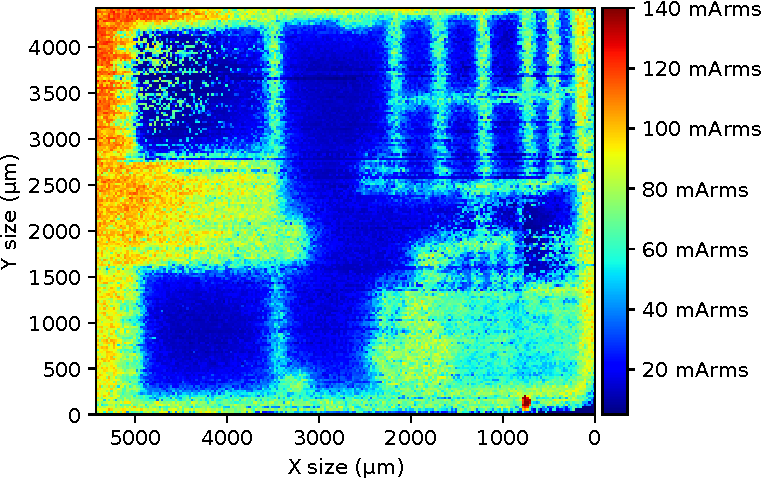
\includegraphics[width=\columnwidth]{./figures/pos_neg_IGND.pdf}
	\caption{Ground current mapping of our target IC}
	\label{stm_ignd}
\end{figure}

	The experimental results are shown in Fig. \ref{stm_ignd}, and the experimental parameters are the following:
	\begin{itemize}
		\item Negative voltage pulse of 70 V amplitude;
		\item Pulse width of 20 ns;
		\item IC substrate thickness of 50 \textmu m.
	\end{itemize}
	The voltage pulse used is of negative polarity as we have observed a very fast degradation of IC subjected to positive voltage pulses, therefore we decided to avoid them at all cost.
	When analyzing the results, we can notice significant differences in the measured current depending on various regions, and the IC floorplan seems to draw itself on the current map.
	The measured RMS current ranges from 10 mArms to 140 mArms, and as predicted by the simulation results, in the regions where the substrate is of dual-well type, the current is higher than on regions where the substrate is of triple-well type, such as the analog block or the flash control region.
	
	These observations confirm the soundness of the proposed models.
	However, as we have seen previously, these models do not consider the functional nature of the considered ICs: their logic behavior.
	To circumvent this limitation, we decided to develop an addition to the initial simulation flow, thus the name "hybrid simulation flow".